\documentclass{beamer}
\mode<presentation>
\usepackage{amsmath}
\usepackage{amssymb}
%\usepackage{advdate}
\usepackage{adjustbox}
\usepackage{subcaption}
\usepackage{enumitem}
\usepackage{multicol}
\usepackage{mathtools}
\usepackage{listings}
\usepackage{url}
\def\UrlBreaks{\do\/\do-}
\usetheme{metropolis}
%\usecolortheme{lily}
\setbeamertemplate{footline}
{
  \leavevmode%
  \hbox{%
  \begin{beamercolorbox}[wd=\paperwidth,ht=2.25ex,dp=1ex,right]{author in head/foot}%
    \insertframenumber{} / \inserttotalframenumber\hspace*{2ex} 
  \end{beamercolorbox}}%
  \vskip0pt%
}
\setbeamertemplate{navigation symbols}{}

\providecommand{\nCr}[2]{\,^{#1}C_{#2}} % nCr
\providecommand{\nPr}[2]{\,^{#1}P_{#2}} % nPr
\providecommand{\mbf}{\mathbf}
\providecommand{\pr}[1]{\ensuremath{\Pr\left(#1\right)}}
\providecommand{\qfunc}[1]{\ensuremath{Q\left(#1\right)}}
\providecommand{\sbrak}[1]{\ensuremath{{}\left[#1\right]}}
\providecommand{\lsbrak}[1]{\ensuremath{{}\left[#1\right.}}
\providecommand{\rsbrak}[1]{\ensuremath{{}\left.#1\right]}}
\providecommand{\brak}[1]{\ensuremath{\left(#1\right)}}
\providecommand{\lbrak}[1]{\ensuremath{\left(#1\right.}}
\providecommand{\rbrak}[1]{\ensuremath{\left.#1\right)}}
\providecommand{\cbrak}[1]{\ensuremath{\left\{#1\right\}}}
\providecommand{\lcbrak}[1]{\ensuremath{\left\{#1\right.}}
\providecommand{\rcbrak}[1]{\ensuremath{\left.#1\right\}}}
\theoremstyle{remark}
\newtheorem{rem}{Remark}
\newcommand{\sgn}{\mathop{\mathrm{sgn}}}
\providecommand{\abs}[1]{\left\vert#1\right\vert}
\providecommand{\res}[1]{\Res\displaylimits_{#1}} 
\providecommand{\norm}[1]{\lVert#1\rVert}
\providecommand{\mtx}[1]{\mathbf{#1}}
\providecommand{\mean}[1]{E\left[ #1 \right]}
\providecommand{\fourier}{\overset{\mathcal{F}}{ \rightleftharpoons}}
%\providecommand{\hilbert}{\overset{\mathcal{H}}{ \rightleftharpoons}}
\providecommand{\system}{\overset{\mathcal{H}}{ \longleftrightarrow}}
	%\newcommand{\solution}[2]{\textbf{Solution:}{#1}}
%\newcommand{\solution}{\noindent \textbf{Solution: }}
\providecommand{\dec}[2]{\ensuremath{\overset{#1}{\underset{#2}{\gtrless}}}}
\newcommand{\myvec}[1]{\ensuremath{\begin{pmatrix}#1\end{pmatrix}}}
\let\vec\mathbf

\lstset{
%language=C,
frame=single, 
breaklines=true,
columns=fullflexible
}

\numberwithin{equation}{section}

\title{MatGeo Assignment Presentation}
\author{Agamjot Singh,\\EE24BTECH11002,\\IIT Hyderabad.}

\date{\today} 
\begin{document}

\begin{frame}
\titlepage
\end{frame}

\section*{Outline}
\begin{frame}
\frametitle{Table of Contents}
\tableofcontents
\end{frame}

\section{Problem}

\begin{frame}
\frametitle{Problem Statement}
Sketch the region $\brak{x, 0} \colon y = \sqrt{4 - x^2}$ and $x$-axis. Find the area of the region using integration.
\end{frame}

\section{Solution}

%Slide1
\subsection{General Equation of Circle and Variable Description}
\begin{frame}
\frametitle{General Equation of Circle and Variable Description}

The general equation of circle is given by

\begin{align}
\label{eq:gen_eq_circle}
\norm{\vec{x}}^2 + 2\vec{u}^{\top}\vec{x} + f = 0
\end{align}

\begin{table}[h!]
	\centering
	\begin{tabular}[12pt]{ |c| c|}
    \hline
    \textbf{Variable} & \textbf{Description}\\ 
    \hline
	$\vec{A}$ & Point to be found\\
    \hline
	$\vec{B}$ & $(0, 0)$ point\\
    \hline
	$\vec{C}$ & $(6, 0)$ point\\
    \hline
	$\vec{\angle \vec{ABC}}$ & $60 \degree$\\ 
    \hline
    \end{tabular}
	\label{tab9.2.35}
\end{table}

\end{frame}

%Slide2
\subsection{Equation of given circle as a general equation in matrix form}
\begin{frame}
\frametitle{Equation of given circle as a general equation in matrix form}

The given curve $y = \sqrt{4 - x^2}$ is that of a semicircle, since $y \geq 0$.
%\newline
The equation of the curve can be written as
\begin{align}
	x^2 + y^2 - 4 = 0, y \geq 0
\end{align}
By comparing with equation $\brak{\ref{eq:gen_eq_circle}}$, the parameters of the circle are
\begin{align}
	\vec{u} = \myvec{0\\0}, f = -4 \implies r = 2, \vec{O} = \myvec{0\\0}
\end{align}

\end{frame}

%Slide3
\subsection{Expressing boundary of $D$ in parametric form}
\begin{frame}
\frametitle{Expressing boundary of $D$ in parametric form}

Boundary of $D$ is the semicircle of radius $r$, which we can parameterize \brak{\text{in counter clock-wise orientation}} using
\begin{align}
	\myvec{x\\y} = \myvec{r\cos{t}\\r\sin{t}}, 0\leq t \leq \pi
\end{align}

\end{frame}

%Slide4
\subsection{Using Green's theorem to find area using line integeral}
\begin{frame}
\frametitle{Using Green's theorem to find area using line integeral}

\textbf{Green's Theorem:}
\newline
Let $C$ be a curve in the plane, and $D$ be the region bounded by it. If $L$ and $M$ are the functions of $\brak{x, y}$ defined on an open region containing $D$, then
\begin{align}
  \oint_{C} \brak{L\, dx + M\, dy} = \int \int_{D} \brak{\frac{\partial{M}}{\partial{x}} - \frac{\partial{L}}{\partial{y}}} \, dA
\end{align}
In this case, to find the area of the region $D$, we substitute $L = -\frac{y}{2}$ and $M = \frac{x}{2}$, then
\begin{align}
\label{eq:greens_theorem}
  \frac{1}{2} \oint_{C} \brak{x\, dy - y\, dx} = \int \int_D \, dA = \text{area of region } D
\end{align}
\end{frame}

%Slide4
\subsection{Calculating the area using line integral}
\begin{frame}
\frametitle{Calculating the area using line integral}

By Green's Theorem $\brak{\ref{eq:greens_theorem}}$,
\begin{align}
	\text{area of D}  = A &= \int \int \, dA\\
	&= \frac{1}{2} \int_{C} x\, dy - y\, dx\\
	&= \frac{1}{2} \int_{0}^{\pi} r^2\brak{\cos^2{t} + \sin^2{t}} \, dt\\
	&= \frac{r^2}{2} \int_{0}^{\pi} \, dt\\
	&= \frac{\pi r^2}{2}\\
	&= 2\pi
\end{align}

\end{frame}

%Slide5
\subsection{Graph}
\begin{frame}
\frametitle{Graph}

\begin{figure}[h!]
   \centering
   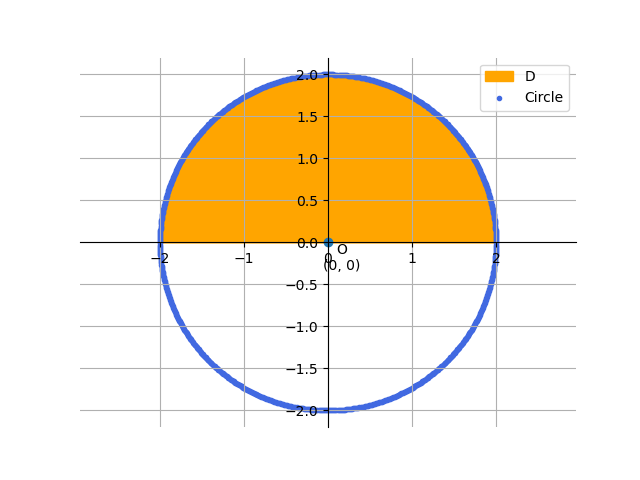
\includegraphics[width=0.7\linewidth]{figs/graph.png}
   \caption{Shaded area representing area of region given}
\end{figure}

\end{frame}

%Slide6
\subsection{C Code}
\begin{frame}[fragile]
\frametitle{C Code}

C function for getting '$n$' number of points to graph a circle of radius $r$ and center $\brak{x, y}$:

\begin{lstlisting}[language=C]
float **circleGet(int n, float x, float y, float r) {
    float **pts = (float **) malloc(sizeof(float *) * n); 
    float theta = 0;
    for(int i = 0; i < n; i++){
        pts[i] = (float *) malloc(sizeof(float) * 2 * n);
        pts[i][0] = x + r*cos(theta);
        pts[i][1] = y + r*sin(theta);
        theta += 2*PI/n;
    }
    return pts;
}
\end{lstlisting}

\end{frame}

%Slide7
\subsection{Python Code}
\begin{frame}[fragile]
\frametitle{Python Code}

The python code for generating the graph can be found at:
\begin{lstlisting}
https://github.com/agamjotsingh1/EE1030/blob/main/matgeo_questions/q9/codes/graph.py
\end{lstlisting}

\end{frame}
\end{document}
